\chapter{绪论}
\section{研究背景及意义}
% \textcolor{red}{正文大概12/65页,最后需要调整一遍格式}

% \textcolor{red}{问题用红色标出,重复用蓝色标出}

% \textcolor{red}{简要说明此项研究工作的目的意义、范围、相关领域的国内外研究现状及前人研究情况和成果(或属知识空白)、理论分析及依据、研究设想、研究方法等,一般不超过全文篇幅的15%。}

% 图的大小一般为宽6.67×高5.00cm。特殊情况下,也可宽9.00×高6.75cm,或宽13.5×高9.00cm。总之,一篇论文中,同类图片的大小应该一致,编排美观、整齐。

% 式中:
% E —— 杨氏模量/GPa;

% 一律使用三线表,与文字齐宽,线粗1磅。

% TODO: 辐射源部分内容仍然较少。
% NOTE: 正文大概65页,在参考文献前,目前52页。
% 第一章 7 页 (第一部分可以先完成,天波部分等英文文章的绪论)
% 第二章 10 页
% 第三章 22 页
% 第四章 12 页
% 第五章 2 页(done)
% NOTE: 问题用红色标出
随着科学技术的进步,现代战场形势瞬息万变,信息对抗在现代军事中的作用越来越重要。纵观整个 20 世纪所爆发的两次世界大战和数次局部战争、21 世纪初的美阿、美伊之战以及最近闹得沸沸扬扬的韩国的萨德事件,无一不昭示着现代战争在很大程度上是信息战。信息战的一个重要特征是利用各种探测、感知手段,借助计算机网络、通信技术,对敌人的作战不对情况做到精确的探测评估,做到“知己知彼,百战不殆”。在信息化战争中,对于空间信息探测、敌方势力的识别、跟踪、定位等功能,主要依靠电子技术来完成\cite{顾耀平2006电子战发展趋势分析, 孙德海2003国外电子战发展综述及对我国电子战研究的思考, 炜森1996综合电子战新技术新方法, 孙纪尧2014电子战}。

在现代电子战信息获取和处理技术中,自动目标识别(Automatic Target Recognition, ATR)是一个十分重要的方面。其主要指的是利用雷达、声波探测等各种主动、被动传感器获取各种信息,然后利用信号处理等方法对这些信号进行分析,从中检测识别出感兴趣的目标或是对于周围环境信息的感知识别。

远程预警是信息战的一个重要部分,需要完成对地平线一下的大型舰船、飞机、导弹等远距离空中或者海中的高价值运动目标的探测,提供远程监视及对关注的空域或者海域目标的检测与跟踪。由于天波超视距雷达(Over-the-Horizon-Radar, OTHR)利用电磁波在电离层间的反射传输高频能量,具有反隐身、抗干扰等有点,其预警能力远远超出常规体制雷达,目前受到越来越多的国家的关注。

信息战的另一个部分是电子情报侦察系统,其主要用途是获取雷达信号的参数情报和战场情报。信号识别的目的就是要详细地了解信号环境中所有雷达信号的特征参数,从中进一步判断这些雷达的用途、平台类别,进而判断其武器系统以及威胁等级,为战略情报分析提供信息。敌方雷达及其武器系统获取有用信息,通过雷达辐射源个体识别,可以对战场环境中敌我双方雷达辐射源的分布情况实施侦察,提供更加全面的、精确的电磁斗争与武器的态势,进行有效的战场指挥与决策,雷达辐射源个体识别已成为当前电子战特别是电子侦察领域的研究热点和难点\cite{matuszewski2008specific}。然而由于辐射源的特征未知、信号波形日趋复杂、战时电磁环境恶劣,给辐射源的精确识别带来了越来越严峻的挑战。

我们可以把上述两个分类识别问题抽象成一个机器学习的问题,也即根据给定的训练数据集学习出一个函数,当新数据到来时,根据这个函数预测出识别结果。具体的机器学习的算法很多,可以通过回归分析和统计分类来构造条件概率,如人工神经网络、决策树等算法。本文基于雷达信号分类中的两个识别问题,对实际数据进行分析,利用深度学习的思想及方法,对天波超视距雷达地海杂波识别以及辐射源的识别进行研究分析,对后续的雷达信号的分类具有一定的理论指导价值和工程借鉴意义。

\section{研究现状}
\subsection{天波超视距雷达地海杂波识别研究现状}
天波超视距雷达利用电磁波在电离层与地/海面之间的反射作用传输高频能量,其作用距离不受地球曲率的限制,可实现对隐身战斗机、洲际导弹、巡航导弹、大中型舰船等高价值目标的远程预警,受到世界各国的高度关注。
天波超视距雷达的主要工作频率为6-28GHz,如图\ref{fig:othr_how}可以通过反射来自电离层的高频(HF)信号来检测和定位1000到3000公里范围内(地平线以外)的飞机或地面目标,因此在持续监测中起着重要作用\cite{headrick1974over, fabrizio2013high}。
然而,电磁信号通过电离层的传播会发生坐标转换,目标处于地面坐标系(即经度和纬度)而天波雷达接收的量测信号则为雷达坐标系下(即斜距和方位角)\cite{krolik1997maximum}。这为雷达的目标跟踪提出了新的需求:坐标配准。
坐标配准是将天波雷达目标从雷达坐标系转换到地理坐标系的过程。天波雷达的坐标配准在很大程度上影响着其跟踪精度,尤其是对于电离层参数无法精确、实时获得的较远的区域。
在这个过程中,我们必须调用两个子过程:(1)如果在雷达坐标系进行目标跟踪,为每个测量或目标状态估计选择正确的电离层传播模式(2)将测量或目标的状态估计从雷达坐标系转换为地面坐标系。
\begin{figure}[htb]
	\centering
	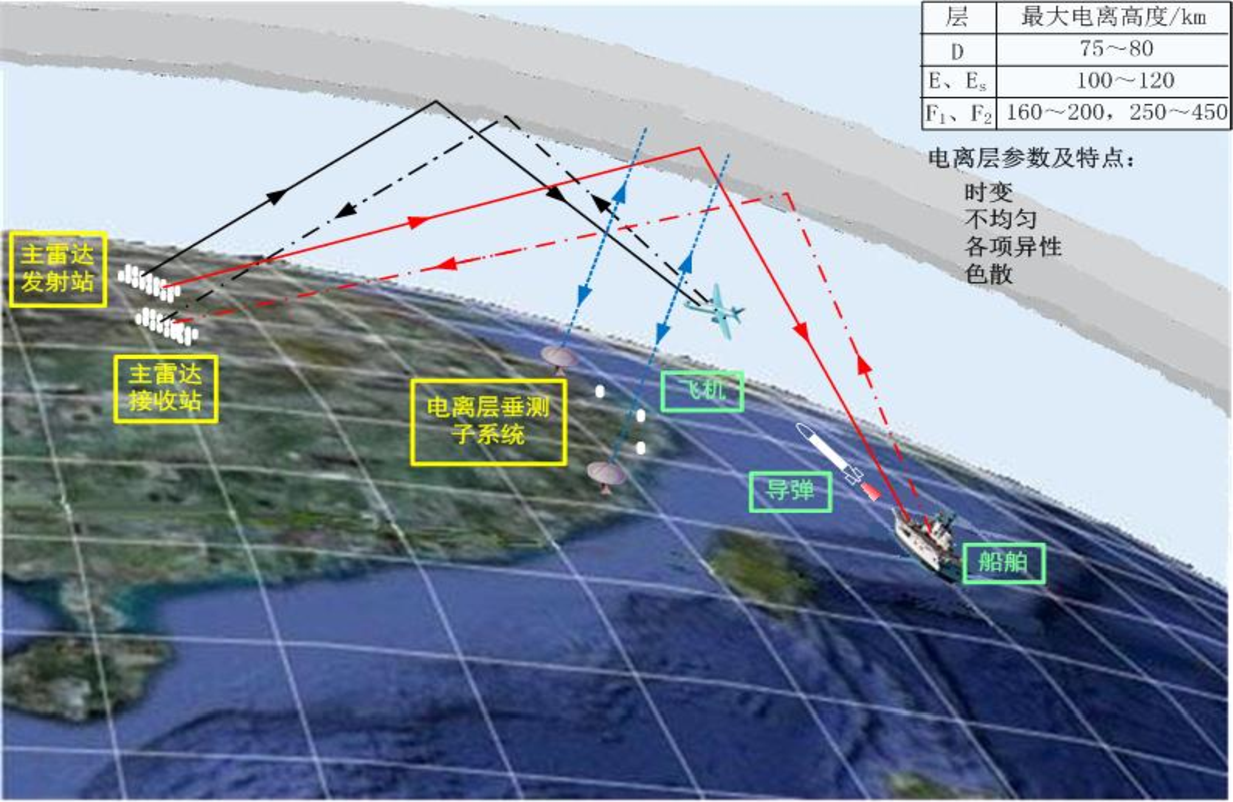
\includegraphics[width=\textwidth]{figures/othr/othr_how}
	\caption{OTHR工作原理示意图}
	\label{fig:othr_how}
\end{figure}

天波超视距雷达由于受雷达工作机制及其电波环境的影响,特别是受电离层多模多路径影响,目标回波-传播模式正确配对很困难,目标检测和定位精度较低。
如图\ref{fig:pdproblem}所示,天波超视距雷达系统主要由主雷达和电离层探测子系统组成,其中后者为前者提供电离层传播条件评估以及坐标配准参数等,如可能的电离层传播模式以及每个模式对应的参数或者电离层的每层高度\cite{wheadon1994ionospheric}。
天波雷达利用这些电离层信息实现坐标配准。然而,利用该方法用两个因素会影响定位的性能:
第一个是探测子系统的部署区域有限,例如该系统无法部署于远海或者敌对区域。对于这些不可探测区域的电离层参数通常是基于统计模型利用已探测区域的参数进行插值求得,但电离层的建模十分复杂且不同区域可能具有较大的变化,这种方式会造成用于坐标配准的电离层参数误差较大,进而影响坐标配准和目标跟踪定位。
第二个是电离层探测子系统独立于主雷达工作导致其提供的坐标配准参数与主雷达存在不一致性问题,例如电离层探测系统识别的传播模式可能不同于天波所接收的量测的传播模式。因此,为了提高电离层传播模式的识别正确率和电离层参数的准确度,进而提高坐标配准的准确性,我们急需一种替代方法。
\begin{figure}[htb]
	\centering
	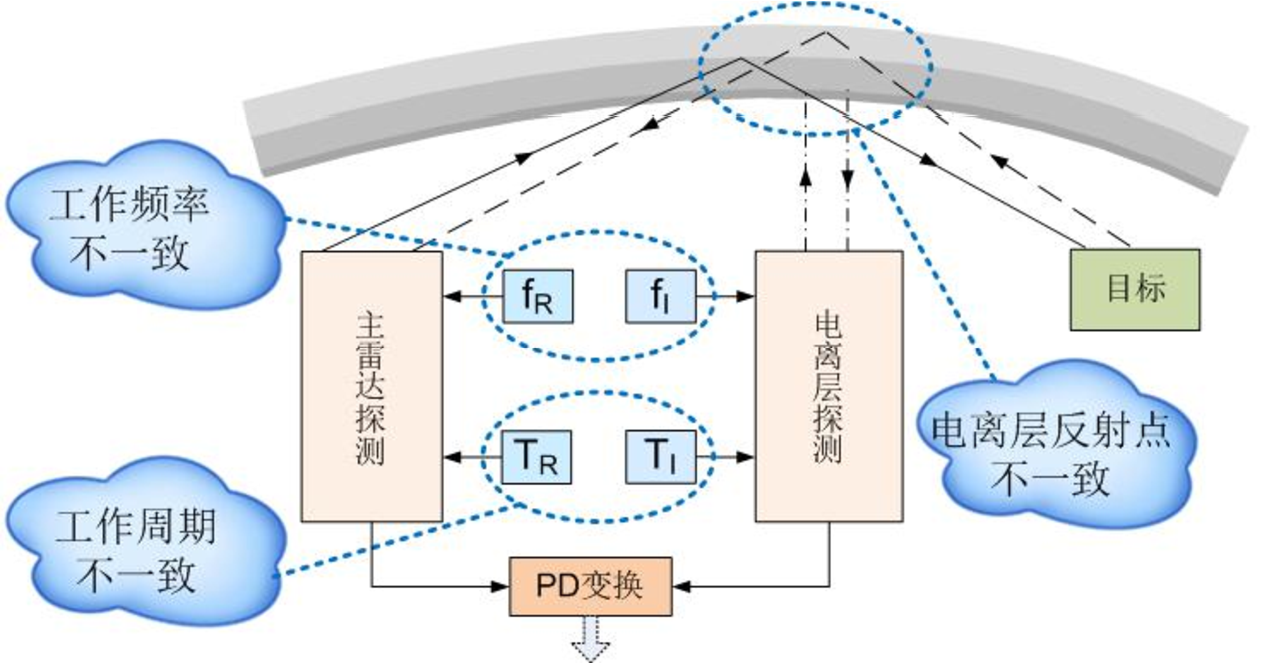
\includegraphics[width=\textwidth]{figures/introduction/pdproblem}
	\caption{环境参数(电离层探测系统)与目标参数(主雷达)不一致}
	\label{fig:pdproblem}
\end{figure}
% 一种改进方式是通过设置有源信标提供坐标配准修正参数,但是受到可部署区域的限制。由于陆地、海洋对雷达信号散射特性不同,可将陆地、海洋地理信息作为一类无源信标。通过区分识别地海杂波、构建地海边界轮廓、与先验地理轮廓信息匹配可同样提供坐标配准修正参数。传统地海杂波识别算法难以准确提取及表达地海杂波特征,从而在复杂电离层状况下地海杂波识别正确率较低。因此,如何发展一种更加准确的地海杂波类型识别方法,对天波超视距雷达电离层参数辨识及目标定位精度的提升有着重要意义。


% 为了提升目标定位经度,一种设想是利用检测区域内的有源/无源信标进行目标位置修正处理,通过对地海杂波特征深入分析和研究,分类识别出地海杂波,提取地海特征信息,并通过与地理位置匹配处理产生修正参数等,从而解决电离层模式配对等诸多工程应用问题,达到提升目标定位精度的目的。同时,在海杂波背景中探测海绵舰船目标的环境极其复杂,由于电波传播环境的影响(电离层时变和失真、易受干扰等),地海杂波附近存在很多虚警回波,严重影响目标的发现和自适应跟踪处理。,既能有效抑制虚警杂波,又能识别出感兴趣的低速舰船目标并稳定跟踪。
针对于该问题,有两种传统的解决方法。
一种方法是利用建立基于先验信息的电离层统计模型,另一种方法是通过一些检测设备收集信息。
Weijers\cite{weijers1995oth}提出了一种利用信标来改善坐标配准的方法。天波雷达接收信标发送的信号,并在雷达坐标系中输出其位置上的量测值。通过将信标的量测与由GPS提供的地面坐标系中的位置进行比较,可以实时地进行坐标的校正。然而,信标也仅限于部署于有限的区域同时需要对信标进行维护。
Fabrizio等人\cite{fabrizio2016using} 提出了一种使用非合作辐射源在已知参考点产生的雷达回波来提高天波雷达坐标配准精度的方法。其使用澳大利亚Jindalee天波超视距雷达的实验数据对该算法进行了验证。
但是这两种方法都有一些限制,前者无法及时更新,有时会产生严重错误(如天气突变情况),后者需要大量设备,并且不容易将其放置在远海地区。针对于这些问题,广大学者进行了大量的研究。

事实上,我们可以利用远海区域的岛屿等陆地作为无源信标来求取电离层的相关参数。如果可以准确的辨识出信号来自陆地还是海洋,可以利用相同的思路进行坐标配准。这种方法的主要思路是,首先通过对于频谱数据的分析识别出每个距离方位分辨单元上的地海情况。然后将识别结果中的地海轮廓与先验的地图轮廓信息进行匹配,匹配过程中的偏差可以作为坐标配准的参数。这种方法最重要的一点就是识别出杂波类型,也就是识别每一个分辨单元是地面还是海洋。
这种方法主要有两个优点。第一个是我们可以使用获得的杂波地形图来匹配实际地图,然后根据匹配结果计算偏移量,从而提高目标跟踪的准确性,另一方面,我们可以通过使用由识别结果获得的频谱上的偏移来校正频谱本身,以提高目标检测的概率和准确度。

使用海岸线的坐标配准的想法首先出现在文\cite{wheadon1994ionospheric, anderson1995auto}中,然而该文并没有给出具体的思路以及实际数据的验证,只是提出了这种思路。Barnum等人\cite{barnum1998over}提出了一种基于地海杂波识别的坐标配准方法,其主要通过构造杂波模型进行杂波识别。然而,由于电离层状况的复杂性,地海杂波杂乱的特征不稳定,例如海杂波的主要特征布拉格峰可能会偏移甚至失去一个峰值。

Cuccoli\cite{cuccoli2009over, cuccoli2009over2, cuccoli2010sea, cuccoli2011coordinate}研究了利用OTHR监测区域地貌结构来进行坐标配准的问题。
对地理信息中的地海用二进制进行表示,然后通过等效的电离层反射高度转换为参考信号。通过最大化接收到的雷达回波与地标特征之间的相关性来确定等效的电离层反射高度。然而,他们假设天波雷达传输单脉冲信号,并提供数值模拟结果。

Cacciamano\cite{cacciamano2012coordinate}等人提出了利用3D射线跟踪算法进行坐标配准误差评估的方法。其主要思想是计算地海分界处的相对群延时与我们先验已知的实际群延时之间的差异进行坐标配准,其中实际的群延时是通过3D射线跟踪算法得到。Holdsworth \cite{holdsworth2017skywave} 提出了一种利用地表回波的反向散射强度,提高目标定位精度的坐标配准方法。\cite{weijers1995oth, fabrizio2016using, wheadon1994ionospheric, anderson1995auto, cuccoli2009over, cuccoli2009over2, cuccoli2010sea, cuccoli2011coordinate, cacciamano2012coordinate}的工作均没有考虑地海杂波的识别问题。

% \textcolor{red}{
% 我们可以根据频谱数据识别出地海分界线,进而确定出岛屿在雷达坐标系中的位置,然后将其与地理坐标中的岛屿对应。因此,我们可以根据相同位置基准的偏差来获得PD变换系数。因此,这种方法最基础和最关键的部分是识别地海杂波识别。
% }

上述所有作者的研究重点主要是如何通过地理坐标的匹配来进行求取变换系数,而对于地海杂波识别方面的研究却并不多。
如图\ref{fig:clutterproblem}所示,利用杂波的频谱数据进行地海杂波识别具有很多特殊的挑战。首先是杂波模型的复杂度,也就是说对于杂波的建模是十分复杂的,这是因为杂波模型随着时间、地点、天气等的变化会发生较大的变化。传统的统计方法中,有多种分布来描述雷达杂波,如瑞利分布(Rayleigh distribution),威布尔分布(Weibull distribution),K分布(K distribution)等,但这些分布均只适用于某些情况,而不能在所有情况下均保持良好的效果。其次,地海杂波的特征无法很好的进行形式化描述。有经验的研究人员可能很容易地根据杂波图区分出某些单元是地还是海,但是用数学方法准确地描述这些特征几乎是不可能的。
\begin{figure}[htb]
	\centering
	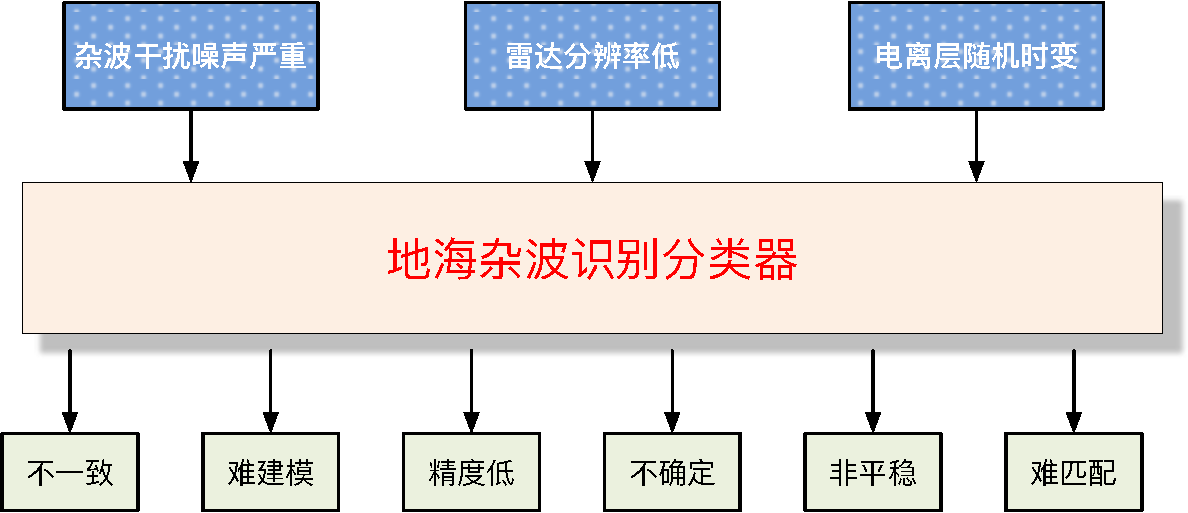
\includegraphics[width=\textwidth]{figures/othr/othr_classification.pdf}
	\caption{地海杂波识别分类器的背景}
	\label{fig:clutterproblem}
\end{figure}
根据我们查阅的参考文献,只有Turley\cite{turley2013high} 和 Jin\cite{jin2012svm}的工作对地海杂波的识别进行了研究。在文 \cite{turley2013high}中,\textcolor{red}{峰值多普勒频谱和布拉格比率检验统计量的多普勒频移测量被用来分类地表回波(陆地或海面后向散射)。 在相邻距离方位角单元的基础上构建图边方程,采用加权最小均方算法(weighted least-mean-square)求解该方程组。}Jin等人\cite{jin2012svm} 提出了一种一种基于支持向量机(Support Vector Machine,SVM)的地海杂波识别的算法。他们通过使用三种地海杂波频谱特征来训练SVM,并用仿真数据进行验证,并且取得了比较好的精度。然而,在实际情况下,地海杂波的特征取决于当时的电离层环境、雷达的扫掠角度、天气环境等,地海杂波模型有十分强的不确定性。当建模所需的参数变化时,算法的准确性将急剧下降。

如图\ref{fig:othr_tradition},OTHR常规地海杂波识别算法采用电离层建模、特征提取、分类的方法,但存在电离层建模复杂以及信息利用不充分的问题。
\begin{figure}[htb]
	\centering
	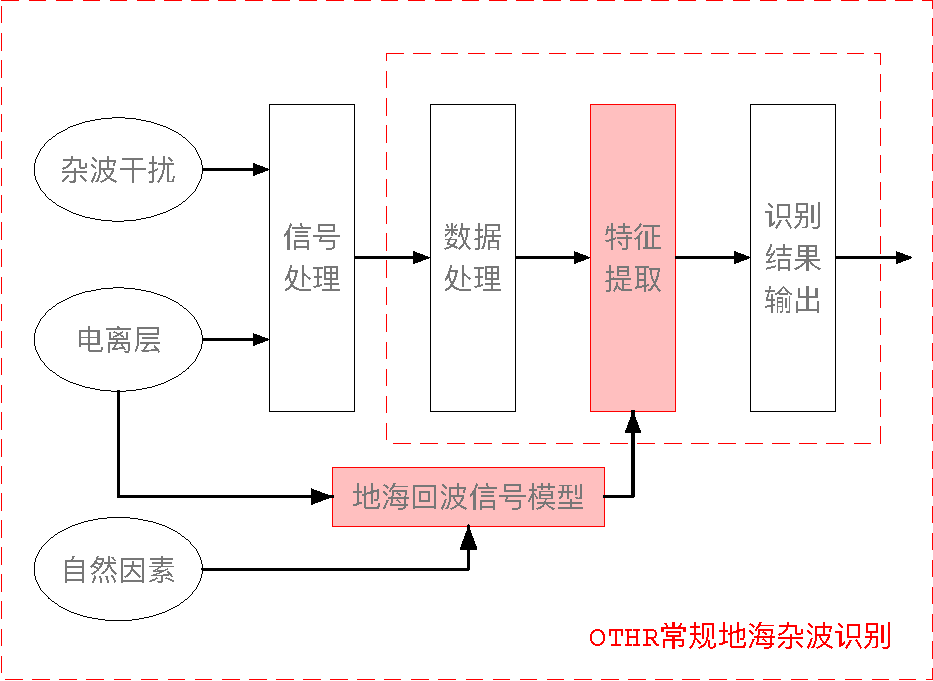
\includegraphics[width=\textwidth]{figures/introduction/othr_tradition}
	\caption{OTHR 常规地海杂波识别}
	\label{fig:othr_tradition}
\end{figure}

% 为了在传播模式不确定、杂波和噪声环境中实现快速准确的地海杂波识别,我们有必要研究新的地海杂波识别的方法。 


\subsection{辐射源个体识别研究现状}
辐射源个体识别(Specific emitter identification, SEI)是一种仅仅依靠发射的无线信号用来辨识出甚至是同一型号的辐射源的技术\cite{Talbot2003Specific}。文献\cite{danev2012physical}表明由于射频(radio frequency,RF)电路硬件在生产制造过程中存在公差并且使用过程中由于使用时间以及工作方式的不同,我们可以通过某种方式识别出不同的辐射源。

辐射源的快速、准确和鲁棒的自动目标识别在现代军事尤其是军事通讯中的作用十分重要\cite{wiley2006elint},尤其是近几年随着认知雷达\cite{kim2008specific}和自组织网络\cite{zhang2013self}等新技术的出现,它已经变得越来越重要。我国在跟踪发达国家研究进展的基础上也开始加紧研发可装备于军方的SEI系统,以逐步缩小与发达国家在技术实用方面的差距。但总体来说,我国在该方面的研究还赶不上美英等发达国家,除了缺乏深层次且系统化的理论分析研究外,更缺乏成熟的工程化系统实践和实际装备,因而迫切需要加快在该领域的理论研究和应用步伐。

辐射源识别是通过将接收到的信号携带的特征与分类的特征组进行比较并选择与这些特征最匹配的类别来区分单个辐射源的过程。因此,
辐射源识别中使用的一种典型方法是维护一个唯一标识各种辐射源的信号特征集,并将辐射源的输入信号与特征集进行比较。将与输入信号最匹配的特征集的标识符(或标签)分配给它\cite{Talbot2003Specific,Zanetti2012Exploring}。
这种方法的隐含要求是特征集合集合。这意味着来自辐射源个体的特征值对于由辐射源产生的所有信号是相似和可重复的,而与由不同辐射源产生的特征值明显不同\cite{Talbot2003Specific}。
根据上述分析,我们可以发现辐射源个体识别的关键技术主要是两部分,一部分是雷达辐射源信号的特征挖掘与提取,另一部分是利用提取的特征进行分类识别。

在雷达辐射源信号特征挖掘与提取方面,国内外很多学者针对此问题作了大量研究工作,在上世纪70年代国外相关研究人员就开始了该部分的研究\cite{therrien1974application},国内的研究始于上世纪80年代初,虽然起步较晚,但受到了军方的高度重视,在“九五”、“十五”和“十一五”国防预研中给予了大力资助。该部分研究主要可以分为两个阶段:

第一阶段为辐射源基本参数特征研究。对于原始信号特征直接求取其载波频率、脉冲宽度、脉冲幅度、到达角度和到达时间等信息\cite{徐欣2001雷达截获系统实时信号分选处理技术研究},利用其中一个或多个作为特征向量。这种情况主要是应用于电磁环境相对单一、辐射源类别较少、信号形式单一、雷达参数固定的早期。

第二阶段为雷达辐射源信号的脉内特征挖掘。当仅仅利用雷达辐射源的参数无法进行准确的辨识的时候,
国内外学者开始研究雷达辐射信号的脉内特征,相继提出了多种分析雷达信号脉内特征的方法。
根据辐射源的操作模式,信号可以分为瞬态信号和稳态信号两种。瞬态信号,通常被称为开启信号,提供了独特和可区分的特征,适合特征提取和辐射源识别\cite{choe1995novel,ureten2005bayesian}。测量瞬态特征的主要方法是通过检测噪声的起始点和终点来从噪声中提取瞬态信号\cite{huang2000bayesian}。基本上,瞬态特征是辐射源特定且一致的,这对于识别是十分有帮助的;然而,由于瞬态信号的持续时间非常短,所以它们很难被捕获。此外,瞬态特征很容易受到非理想和复杂的信道条件的阻碍,这可能对识别结果产生负面影响\cite{xu2007identification}。

稳态信号由在稳定条件下工作的辐射源传输。尽管稳态特征倾向于被传输的信息破坏,导致提取它们的困难,但是稳态信号的识别具有相当大的实际意义,因为其很容易被检测和捕获。在这种情况下,已经研究了许多特征提取方案,
最先被提出的是对于时域信号进行分析处理的方法,如Roe提出的时域波形分析法\cite{roe1994real};继而学者利用频域信号进行挖掘,如谱相关法\cite{jouny1995radar,zhang2001new}、脉内瞬时频率特征\cite{kawalec2004radar,毕大平2005基于瞬时频率的脉内调制识别技术}与累积法\cite{aubry2011cumulants}、普运伟提出的瞬时频率派生特征\cite{普运伟2009雷达辐射源信号瞬时频率派生特征分类方法},随后学者同时综合时域信息与频域信息提出了时频综合法\cite{chen1999joint,li2011quadratic,moraitakis2000feature},时频表示将信号映射到二维时间和频率平面上,同时提供时间和频谱信息。在\cite{lopez2005digital}中,基于短时傅立叶变换(short-time Fourier transform, STFT)提出了一个信号检测和识别系统。然而,STFT是不能用于分析非线性信号的线性变换。
小波分析因其多分辨率分析的特点也被广泛应用于该领域,Cohen\cite{cohen2002importance}首次将小波变换引入到信号的分析处理,余志斌在此基础上提出了基于局域波分解\cite{余志斌2008基于局域波分解的雷达辐射源信号时频分析}、小波脊频级联特征\cite{余志斌2010一种新的,余志斌2010基于小波脊频级联特征的雷达辐射源信号识别}的脉内特征挖掘方法和小波包特征\cite{张葛祥2006基于小波包变换和特征选择的雷达辐射源信号识别}等;
越来越多其余学科的知识也被应用于该领域,如信息理论准则与聚类技术综合法\cite{zhou1999combining}、信号的分形特征等\cite{dudczyk2013identification,zhang2003fractal,dudczyk2013fractal}、基于Chirplet原子的特征\cite{朱明2009一种基于}、熵特征\cite{张葛祥2005基于熵特征的雷达辐射源信号识别}、粗集理论\cite{张葛祥2005基于粗集理论的雷达辐射源信号识别}、信息维数\cite{张葛祥2005雷达辐射源信号智能识别方法研究}和分形盒维数\cite{张葛祥2003雷达辐射源信号分形特征研究,张葛祥2004雷达辐射源信号脉内特征分析}等来量化评估信号的不确定性和复杂性。

另一方面,雷达辐射源识别是一个典型的分类问题,其主要思路为在得到辐射源信号的特征表示之后,借助有效的分类算法来实现特征空间到决策空间的转换,从而确定信号的所属类别。
总体上有三种分类方法被应用于雷达辐射源识别中:一种是决策树分类算法,通过人类专家的先验知识进行分类,如ID3\cite{lyden1999id1}、C4.5算法\cite{quinlan1996bagging}和模板匹配\cite{dudczyk2015fast,dudczyk2004applying}等;
另一种为生成模型分类器,其主要是基于先验概率和类别条件概率密度进行估计,如K最近邻算法\cite{cover1967nearest}。
第三种是判别型分类器,其需要在学习过程中最优化某种目标函数,如线性判别分类器\cite{mika1999fisher}、神经网络\cite{jouny1993classification,petrov2013identification,shieh2002vector,willson1990radar}、支持向量机\cite{ren2008radar}等方法。

从目前的研究现状来看,大多数研究方法存在三个主要缺陷:
\begin{itemize}
	\item 特征提取过程计算量大,需要大量的存储空间;
	\item 特征选择比较困难:不同的特征在分类识别能力上存在差异;
	\item 目前的研究重点主要集中在不同调制类型的辐射源的识别方面,而关于参数不同或者参数相近乃至相同的辐射源识别的研究较少,限制了其实际应用;
	\item 目前的分类识别局限于已知类别的识别,当有新的来自未知类别的辐射源出现时,无法准确迅速的发现;
\end{itemize}


% \textcolor{red}{添加详细的描述,类似于上一节}

\subsection{深度卷积神经网络在雷达信号处理中的应用}

由于深度卷积网络在图像、语音等领域的卓越表现,一部分学者也开始将其应用于雷达的信号处理领域。在早前,大部分应用均集中于合成孔径雷达(Synthetic aperture radar,SAR)图像识别,主要用于遥感中的地物分类领域\cite{chen2014sar,xie2014multilayer,lv2014classification}。Xie \cite{xie2014multilayer}基于深度学习提出了一种自动学习极化合成孔径雷达(PolSAR)中多层特征的方法。文中主要利用了叠加稀疏自编码器(SAE),使用少量标签微调他们的方法的参数。最终,实验结果证实了其所提出的方法在分类精度和视觉效果方面具有显著的提升。

而随着深度学习技术的发展,一部分学者逐渐把深度学习引入新的领域。恒虚警 (Constant False Alarm Rate, CFAR)检测是雷达系统常用的目标检测算法,传统的方法可以分为几种在不同环境下具有不同性能的方法。Rohman \cite{rohman2017classification}提出了一种隐含神经元数变化的集成神经网络分类器,对雷达环境进行分类的自适应CFAR检测方法。在多目标和杂波边界环境下,该方法仍然能够表现出最好的性能。Kim提出了一种基于多普勒雷达的深度卷积神经网络(DCNNs)用于人体检测和活动分类的方法\cite{kim2016human}。 他们主要针对传统解决方案中依赖于手工特征的设计这个问题,提出了将DCNN直接应用于人体检测和活动分类问题的原始多普勒频谱图。DCNN可以使用测量数据共同学习必要的特征和分类边界,而不需要在多普勒信号上使用任何明确的特征,并且取得了很高的精度。Zhang \cite{zhang2017novel}针对不同运动形式和复杂杂波背景下的多目标跟踪问题,通过将传统的MN逻辑航迹起始算法与深度学习进行结合实现了在复杂杂波环境下的多目标航迹起始算法。仿真实验表明,其方法比传统的用于航迹起始的改进Hough变换要好得多,特别是在目标机动的情况下,同时该方法具有很强的鲁棒性和适应性,能够对来自不同雷达的数据进行起始。虽然应用场景逐渐增大,但是大部分的实施步骤仍然是利用二维的卷积神经网络对图像进行分类识别等。
% 我们在此通过对雷达信号序列的分析,利用深度学习方法对一维序列雷达信号进行处理。

\section{论文研究内容及结构}

本文主要研究内容是基于深度学习的雷达信号分类技术,研究重点为深度学习方法在天波雷达地海杂波识别和辐射源分类中的应用。针对于复杂环境下天波雷达地海杂波的不确定性以及在含有未知分类的情况下的辐射源识别两个主要方面进行研究,本文各章安排如下:

第一章为绪论,主要介绍了天波超视距雷达地海杂波识别的意义以及发展,辐射源类别识别的国内外研究现状。

第二章为深度卷积神经网络。该章主要是基本的深度学习理论的相关介绍。

第三章为基于深度学习的地海杂波识别。根据天波超视距雷达的频谱信息,利用一维卷积神经网络作为分类器区分出获取的杂波类型。在实际数据的验证中,即使是在电离层环境很差的情形下,该算法仍然具有很高的精确度。并且将识别结果与实际的地图轮廓进行了匹配,仍然具有很高的匹配率。

第四章为基于深度学习的辐射源未知分类识别。针对于复杂电磁环境下辐射源识别困难的问题,设计了一个深度卷积神经网络,利用模糊函数作为特征实现了对于已知类别的辐射源的识别,同时设计了一个Meta-Recognization,对于识别结果做了进一步的处理,实现了未知分类的辨别。利用实际的雷达数据进行验证,该算法具有很高的识别准确率和分辨正确率。

第五章对全文进行总结,并对后续的研究方向进行了讨论。